\documentclass[conference]{IEEEtran}

\usepackage[UTF8,scheme=plain,fontset=fandol]{ctex}
\usepackage{cite}
\usepackage{amsmath,amssymb,amsfonts}
\usepackage{booktabs}
\usepackage{graphicx}
\usepackage{xcolor}
\usepackage{colortbl}
\usepackage{multirow}
\usepackage{array}
\usepackage{url}
\usepackage{grffile}
\usepackage{balance}

\graphicspath{{figures/method/}{figures/results/}{figures/supplementary/}}
\renewcommand{\refname}{参考文献}

\newcommand{\method}{Alpha-STALLED}
\newcommand{\stall}{STALL}
\newcommand{\sreal}{S_{\mathrm{real}}}
\newcommand{\sglobal}{S_{\mathrm{global}}}
\newcommand{\slocal}{S_{\mathrm{local}}}

\begin{document}

\title{\method：基于全局--局部真实视频校准的免训练生成视频检测}

\author{
  \IEEEauthorblockN{作者姓名待定}
  \IEEEauthorblockA{
    单位待定\\
    邮箱待定}
}

\maketitle
\zihao{-5}
\linespread{1.12}\selectfont

\begin{abstract}
免训练生成视频检测需要从冻结视觉表示中提取有判别力的时间证据。
将局部变化提前汇总为空间平均或少数标量，可能丢失真实分布中有用的方向信息。
本文提出 Alpha-STALLED，在同网格图块特征上构造归一化二阶残差，
先以真实统计度量各位置的变化方向，再聚合局部证据并与全局评分融合。
视觉编码器保持冻结，统计参数仅由真实视频拟合，无需训练真假分类器。
三个基准、23个生成器单元上的三域等权 Average AUC/AP-real 为0.874/0.877，
相对同目标真实信息预算的全局对照提高0.009/0.005。
匹配拟合位置数后，局部方向相对提前空间聚合仍提高0.020/0.021；
更换真实拟合视频后，二阶相对一阶的增量和对全局的平均AUC补充得到重复验证。
这些结果支持先测量局部动态方向、再汇总证据的设计，同时揭示其参考与观察条件依赖。
\end{abstract}

\begin{IEEEkeywords}
生成视频检测，免训练检测，局部动态方向，真实统计度量，二阶差分
\end{IEEEkeywords}

\section{引言}
\label{sec:introduction}

生成视频检测需要应对持续变化的生成模型。
免训练方法复用预训练表示或生成模型的统计特性，避免为每类新生成器训练真假分类器。
近期工作分别从特征变换的稳定性~\cite{choi2025warpad}、
帧间变化~\cite{zheng2025d3,brokman2026overcoherence}及真实参考似然~\cite{benhayun2026stall}
构造检测分数。
这使研究重点从扩大分类器转向一个更具体的问题：冻结表示中的哪些信息，应当以何种方式被测量？

时间线索既可以体现为变化，也可以体现为过度连贯。
D3~\cite{zheng2025d3}度量相邻特征距离的二阶波动，
Over-Coherence~\cite{brokman2026overcoherence}利用局部或整体偏高的帧间相似性，
SPLIT~\cite{hyun2026split}进一步比较图块路径粗糙度与邻接位移。
STALL~\cite{benhayun2026stall}则用真实统计联合解释全局外观和归一化一阶变化。
这些方法确立了时间与局部证据的价值，但尚未替代对
\emph{局部高维二阶方向在真实度量下的增量}的直接检验。

本文的出发点是测量与聚合的顺序。
不同位置的变化可能在空间平均中抵消；具有相同长度的残差，也可能落在真实统计中具有不同代价的方向。
因此，我们在空间汇总前保留各位置的归一化二阶残差，
让真实协方差定义方向度量，再聚合位置评分。
这一设计利用了局部动态分布的信息，同时保留与全局证据共享视觉编码的简单实现。

我们将该方法称为\method。
固定真实参考后，同一套评分规则用于该域的各个生成器；推理无需生成器身份。
局部方向表示、真实统计度量和固定预算片段观察共同构成检测流程，
其中局部方向的补充价值通过匹配对照验证。
本文的贡献为：
\begin{itemize}
  \item \textbf{局部方向的真实统计评分。}
  在冻结表示上先测量逐位置二阶方向、后汇总证据，并解释该顺序保留的方向离散信息。
  \item \textbf{区分表示收益与额外参考支持。}
  在相同真实预算与观察条件下，通过聚合、阶次和位置数控制检验局部增量，并以新真实拟合池验证其重复性。
\end{itemize}

\section{相关工作}
\label{sec:related_work}

\subsection{生成图像与生成视频检测}
早期生成内容检测主要依赖监督式图像分类器或手工伪影特征。随着生成模型快速变化，这类检测器在未见生成器上容易退化。后续方法引入 CLIP、DINO 等预训练视觉特征，以提升跨生成器泛化能力；训练自由图像检测方法进一步尝试通过重建误差、特征一致性或表示空间统计来避免合成样本依赖，例如 AEROBLADE、ZED 和 RIGID~\cite{ricker2024aeroblade,cozzolino2024zed,he2024rigid}。但图像检测器天然是逐帧的，仍然难以直接建模跨帧运动一致性。

生成视频检测同时需要处理空间外观和时序动态。GenVideo~\cite{chen2024genvideo} 和 VideoFeedback/VideoScore~\cite{he2024videoscore} 等数据集推动了生成视频评测，但许多检测器仍依赖监督训练或特定 benchmark。D3~\cite{zheng2025d3} 使用二阶时序特征描述帧间动态差异；Over-Coherence~\cite{brokman2026overcoherence} 利用生成视频帧间过度一致性；\stall~\cite{benhayun2026stall} 则把空间外观和全局帧间差分统一到真实视频似然框架中。近期 SPLIT~\cite{hyun2026split} 进一步在冻结视觉编码器的 patch token 上结合时间粗糙度与局部空间运动不一致，并面向低 FPR 和部分编辑视频评测。本文与这些方法共享 training-free 时序检测背景，但关注的问题是：在 \stall 的真实似然框架中，目标域真实视频校准的同网格 Local D2 是否能稳定补充 Global 证据，以及哪些早期局部分支应通过受控消融删除。

\subsection{白化似然与冻结视觉表征}
白化高斯似然把预训练视觉表征映射到近似各向同性的空间后，以闭式形式估计样本在真实分布下的典型性。该思想已被用于 CLIP 表征的生成图像检测和激活空间统计分析~\cite{betser2025whitenedclip,betser2026conditional,rachmil2025whitening}。\stall 进一步表明，在 DINOv3 全局帧表征中，帧级特征和归一化帧间差分可以被真实视频校准集近似建模，并通过百分位映射得到可比较的空间和时序分数。本文保留这一统计形式，但把被建模对象从全局 token 扩展到 patch token 及其同网格二阶差分。

\subsection{局部时序证据}
局部时序证据在视频取证中具有直接意义：许多生成伪影表现为短时、局部、非语义的变化，例如纹理闪烁、物体边界不稳定或局部运动方向突变。显式光流或 patch 匹配可以描述局部运动，但在生成视频伪影区域容易受到匹配错误影响。本文采用更低假设的同网格策略：不追踪物体，不搜索对应区域，只在冻结 DINOv3 的固定 patch 网格上计算二阶差分。这一选择牺牲了物体级运动解释能力，但提高了协议简洁性和复现性，也与免训练检测目标一致。

需要特别注意，运动型检测器可能利用 real/fake 在 FPS、时长或运动幅度上的数据集偏差。近期统一预处理审计显示，多种运动检测器在 motion rebalancing 或单帧扰动后明显下降~\cite{michels2026biases}。因此本文把同协议 D1/D2、K1/K3 和 Spatial factorial 作为内部因果证据，同时将 motion-balanced 与统一转码评测列为投稿前必须补齐的外部压力测试，而不把当前 benchmark 增益外推为普遍生成痕迹。

\section{方法}
\label{sec:method}

\subsection{任务定义与总体流程}
给定视频 $V=\{I_t\}_{t=1}^{T}$，目标是输出真实性分数 $S(V)\in[0,1]$：分数越高，视频越符合真实视频的统计规律。检测器仅使用预先指定的真实视频建立参考统计，不以生成视频训练分类器，也不在推理时读取生成器来源、测试标签或测试批次的类别构成。真实校准集与目标评测集严格隔离，具体划分见实验设置。

图~\ref{fig:pipeline} 展示了 \method 的两阶段流程。参考构建阶段，真实视频经过冻结的 DINOv3 编码器，得到全局标记与图块标记；随后分别估计全局空间、全局一阶时序、局部空间和局部二阶时序的白化参数，并保存真实视频的分支统计量以进行百分位校准。推理阶段，每个视频在可用时长内均匀选取至多三个互异的 2 秒窗口，每个窗口包含 8 FPS 下的 16 个不同帧。各窗口独立产生全局和局部分数，两个分支分别在视频级取均值、按有效窗口数重新校准，再使用固定权重融合。

\begin{figure*}[!t]
  \centering
  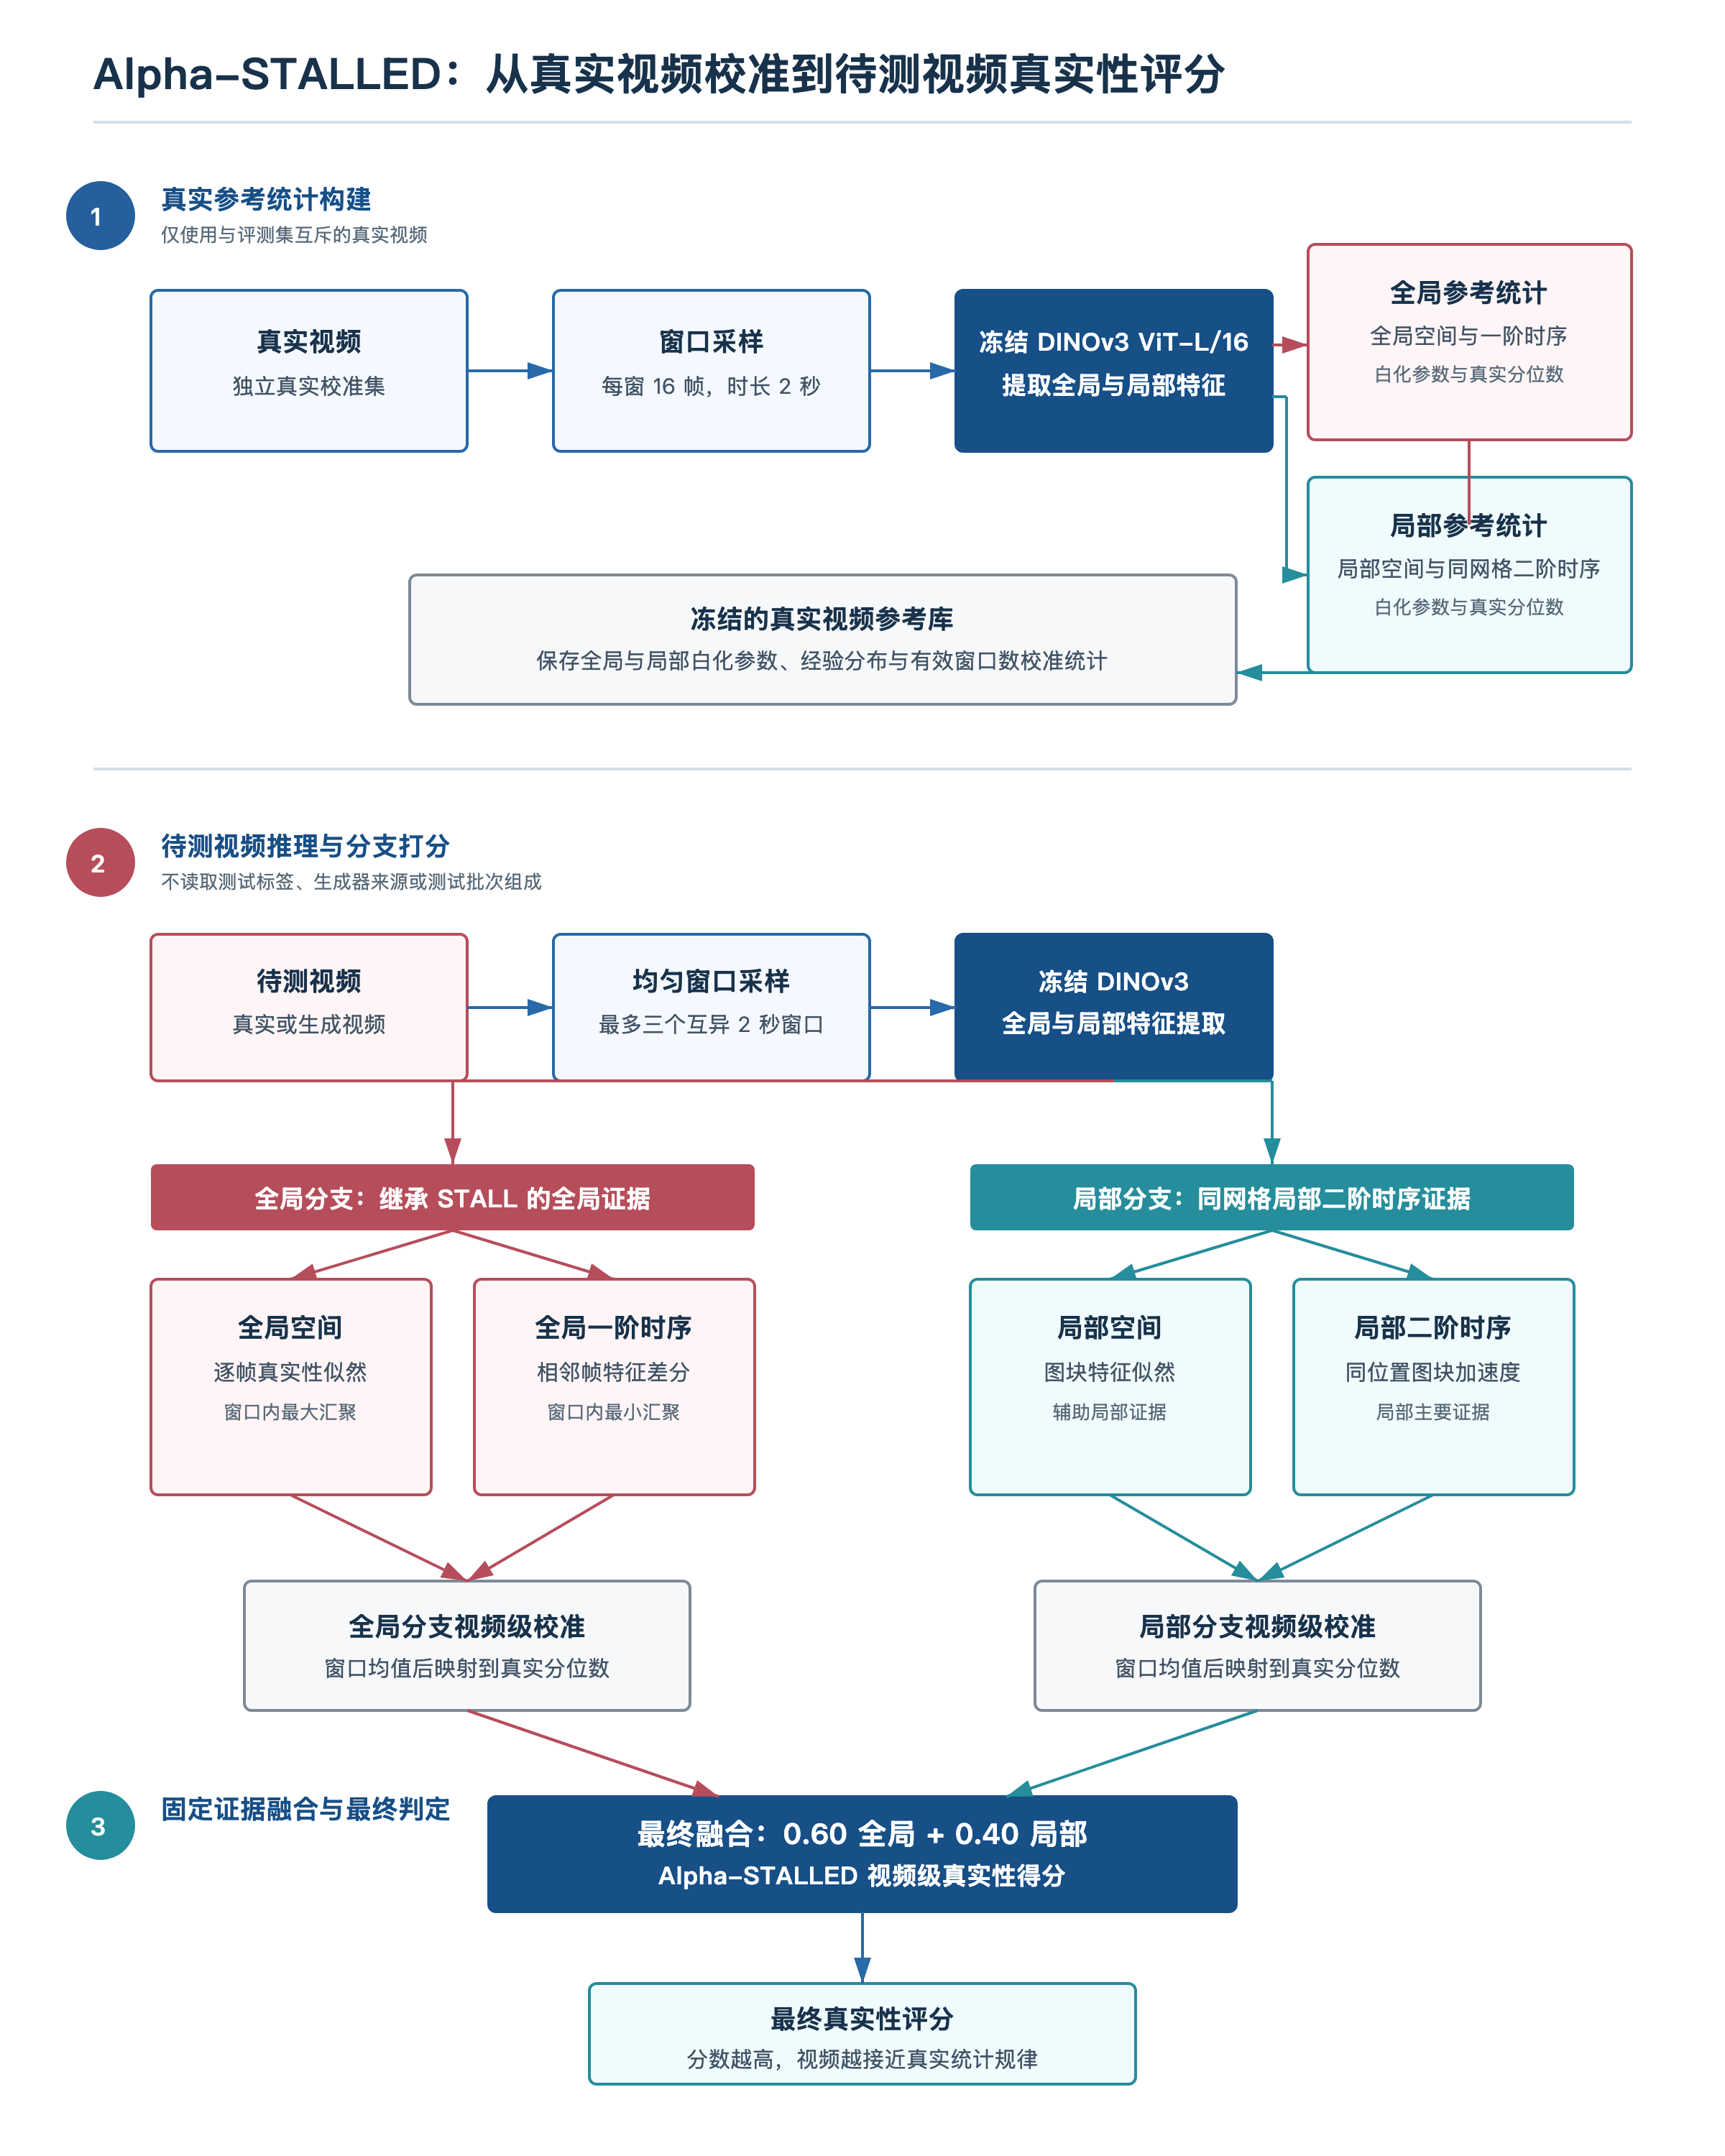
\includegraphics[width=\textwidth,height=0.72\textheight,keepaspectratio]{alpha_stalled_pipeline_zh.png}
  \caption{\method 的全局--局部真实视频校准流程。全局分支继承 \stall 的空间和时序似然；局部分支在 DINOv3 图块标记上建模局部空间似然和同网格二阶时序似然。局部证据先汇聚为统一局部分数，再与全局分数融合。}
  \label{fig:pipeline}
\end{figure*}

\subsection{冻结 DINOv3 表征}
所有分支共享同一个冻结 DINOv3 ViT-L/16 编码器~\cite{simeoni2025dinov3}。第 $t$ 帧输入后得到全局帧表征和 patch token 网格：
\begin{equation}
  g_t\in\mathbb{R}^{D},\qquad
  P_t=\{p_{t,i}\}_{i=1}^{N}\in\mathbb{R}^{N\times D}.
  \label{eq:dino_features}
\end{equation}
本文使用 $D=1024$、$N=14\times14$。全局序列 $G=\{g_t\}_{t=1}^{T}$ 对应 \stall 的全局空间和全局时序分支；局部序列 $P=\{P_t\}_{t=1}^{T}$ 用于构建图块空间与图块二阶时序分支。两类证据共享同一次前向传播，因此局部扩展无需训练额外的骨干网络。

\subsection{白化高斯似然与百分位校准}
对任一分支的特征向量 $x\in\mathbb{R}^{d}$，根据真实校准集估计均值 $\mu$ 和协方差 $\Sigma=U\Lambda U^\top$。保留正特征值对应子空间后，构造白化矩阵：
\begin{equation}
  W=U_r\operatorname{diag}\left((\lambda_1+\epsilon)^{-1/2},
  \ldots,(\lambda_r+\epsilon)^{-1/2}\right),
  \label{eq:whitening}
\end{equation}
其中 $\epsilon$ 是数值稳定项。白化特征及其标准高斯对数似然为
\begin{align}
  z(x)&=(x-\mu)W,\\
  \ell(x)&=-\frac{1}{2}\left[r\log(2\pi)+\lVert z(x)\rVert_2^2\right].
  \label{eq:gaussian_ll}
\end{align}
该分数不是监督分类边界，而是衡量样本是否落在真实视频参考分布的高密度区域。

不同分支的原始对数似然尺度不同，因此本文沿用 \stall 的经验百分位校准。设分支 $b$ 的视频级统计为 $q_b(V)$，真实校准视频的对应统计集合为 $\mathcal{C}_b=\{c_{b,j}\}_{j=1}^{M}$，则
\begin{equation}
  s_b(V)=\widehat F_b(q_b(V))=
  \frac{1}{M}\sum_{j=1}^{M}\mathbb{I}\left[c_{b,j}\leq q_b(V)\right].
  \label{eq:percentile}
\end{equation}
校准后，$s_b(V)$ 越大表示该分支证据越接近真实视频。

\subsection{全局 \stall 分支}
全局空间分支对每帧 $g_t$ 计算空间似然，并以视频内最大空间似然作为统计：
\begin{align}
  \ell^{\mathrm{gs}}_t &= \ell_{\mathrm{gs}}(g_t),\\
  q_{\mathrm{gs}}(V) &= \max_t \ell^{\mathrm{gs}}_t .
  \label{eq:global_spatial}
\end{align}
全局时序分支对相邻全局帧特征差分进行 L2 归一化：
\begin{equation}
  d_t=\frac{g_{t+1}-g_t}{\lVert g_{t+1}-g_t\rVert_2},
  \qquad t=1,\ldots,T-1,
  \label{eq:global_delta}
\end{equation}
随后以最低转移似然作为视频级时序统计：
\begin{align}
  \ell^{\mathrm{gt}}_t &= \ell_{\mathrm{gt}}(d_t),\\
  q_{\mathrm{gt}}(V) &= \min_t \ell^{\mathrm{gt}}_t .
  \label{eq:global_temporal}
\end{align}
本文使用 \stall 的等权全局空间--时序融合规则。经百分位映射后，第 $k$ 个窗口的全局真实性分数为
\begin{equation}
  G_k=0.5s_{\mathrm{gs},k}+0.5s_{\mathrm{gt},k}.
  \label{eq:global_window_score}
\end{equation}

\subsection{局部图块分支}
\subsubsection{局部空间似然}
局部空间分支直接对图块标记 $p_{t,i}$ 建模：
\begin{equation}
  \ell^{\mathrm{ps}}_{t,i}=\ell_{\mathrm{ps}}(p_{t,i}).
  \label{eq:patch_spatial}
\end{equation}
该分支提供局部纹理、结构和边缘异常证据。实验表明，单帧局部外观在跨数据集上通常弱于局部时序证据，因此它被作为局部分数中的辅助证据。

\subsubsection{同网格二阶时序似然}
局部时序分支是 \method 的核心新增模块。为避免显式图块匹配带来的不稳定性，我们固定 DINOv3 的 $14\times14$ 图块网格，不包含 CLS 或注册标记，并在同一空间位置上计算连续三帧的二阶差分。本文不做区域池化，区域大小固定为 1：
\begin{align}
  a_{t,i}&=p_{t+2,i}-2p_{t+1,i}+p_{t,i},\\
  \hat a_{t,i}&=\frac{a_{t,i}}{\lVert a_{t,i}\rVert_2},
  \qquad t=1,\ldots,T-2 .
  \label{eq:patch_acceleration}
\end{align}
该特征刻画局部表征轨迹的加速度。真实视频中的局部纹理和结构通常随时间连续变化，而生成视频中的闪烁、漂移和局部形变突变会使 $\hat a_{t,i}$ 偏离真实参考分布。局部时序似然为
\begin{equation}
  \ell^{\mathrm{pt}}_{t,i}=\ell_{\mathrm{pt}}(\hat a_{t,i}).
  \label{eq:patch_temporal}
\end{equation}

\subsubsection{局部证据聚合}
局部空间和二阶时序似然均在窗口内对时间与图块位置取算术均值。该设置在三个数据集上保持一致，不随数据集改变区域大小、聚合方式或低分图块比例。其余聚合和匹配变体仅用于补充敏感性分析，不构成本文方法。

\subsection{局部分数与全局--局部融合}
经窗口级真实百分位校准后，局部空间分数和局部二阶时序分数组合为
\begin{equation}
  L_k=0.1s_{\mathrm{ps},k}+0.9s_{\mathrm{pt},k}.
  \label{eq:local_window_score}
\end{equation}
局部二阶时序是 Local 的主要证据；PatchSpatial 只保留固定的 0.1 权重，不再进行数据集特定搜索。

设视频 $V$ 的有效窗口数为 $K_V\leq3$。首先分别聚合两个分支，
\begin{equation}
  G_{\mathrm{raw}}(V)=\frac{1}{K_V}\sum_kG_k,\qquad
  L_{\mathrm{raw}}(V)=\frac{1}{K_V}\sum_kL_k.
  \label{eq:branch_video_mean}
\end{equation}
随后使用具有相同有效窗口数的真实校准视频分别建立经验 CDF，得到 $G(V)$ 与 $L(V)$。每个校准视频在每个分支中只贡献一个视频级统计，长视频不会因窗口更多而获得更大权重。最终分数为
\begin{equation}
  S(V)=0.6G(V)+0.4L(V).
  \label{eq:final_score}
\end{equation}
局部白化、窗口级经验分布函数和视频级经验分布函数均仅由目标域的独立真实视频估计；生成视频不参与这些统计量的拟合或校准。$\alpha$、$\beta$、$K$ 与总体结构在三个开发数据集上确定，因此这些数据集不构成独立确认集。实现中，白化和高斯似然计算采用 float64，经验分布函数采用稳定排序及右闭合并列规则；DINOv3 特征仍保持 float32，从而避免高维白化对外层批量形状的数值依赖。

\section{实验}
\label{sec:experiments}

\subsection{设置与指标}
评价涵盖VideoFeedback~\cite{he2024videoscore}、GenVideo~\cite{chen2024genvideo}
和ComGenVid~\cite{benhayun2026stall}，分别包含11、10和2个生成器单元。
采用STALL的动态等级筛选与生成器内真假平衡配对；
Hotshot-XL和MoonValley保留1秒观察。
共包含15,569个带时长的片段身份、14,573个不同视频文件和23,550条配对记录。
拟合、参考及评价按已知源组隔离；同源的不同观察不作为独立源。
原拟合池每域200片段，其中ComGenVid对应132个源，另两域各200源。

报告AUC及以真实为正类的AP（AP-real），数值越高越好。
每域先对生成器等权平均，本文的总体Average再对三个域等权平均。
对本次匹配预测采用1,000次源组配对bootstrap估计95\%区间；
复用真实视频在不同配对中共享抽样权重。
方法设计在这些开发基准上完成；真实统计拟合不使用生成样本，不等于开发过程从未查看生成结果。

\subsection{主要结果}
\begin{table}[!t]
  \centering
  \caption{锁定 \method 与正式方法链条对比。指标为 pairwise balanced AUC/real-positive AP，数值越高越好。}
  \label{tab:main_results}
  \resizebox{\columnwidth}{!}{%
  \begin{tabular}{lcccc}
    \toprule
    方法 & ComGenVid & VideoFeedback & GenVideo & Macro-3 \\
    \midrule
    Original STALL & 0.8508/0.8560 & 0.8449/0.8596 & 0.8206/0.8129 & 0.8388/0.8428 \\
    Clean single-window & 0.8699/0.8819 & \textbf{0.8631/0.8708} & 0.8382/0.8274 & 0.8570/0.8600 \\
    \method (locked K=3) & \textbf{0.8968/0.9064} & 0.8597/0.8689 & \textbf{0.8657/0.8416} & \textbf{0.8741/0.8723} \\
    \bottomrule
  \end{tabular}
  }
\end{table}

% 预先入队，后续正文按表II的A/B/C和表III顺序引用。
% 由 export_tables.py 生成；CSV 身份及汇总经校验。
\begin{table}[t]
  \centering
  \caption{局部分支的受控贡献。每格为 AUC/AP-real，Average 为三域等权。粗体为整表各列各指标的显示最高值（含并列）；浅底色标出冻结的完整方法。}
  \label{tab:component_ablation}
  {\footnotesize
  \setlength{\tabcolsep}{2.2pt}
  \renewcommand{\arraystretch}{1.15}
  \begin{tabular*}{\columnwidth}{@{\extracolsep{\fill}}lcccc@{}}
    \toprule
    配置 & VF & GV & CGV & Average \\
    \midrule
    \multicolumn{5}{@{}l}{\textbf{A. 分支互补}} \\
    $G$ & 0.823/\textbf{0.844} & 0.873/0.863 & 0.900/0.909 & 0.865/0.872 \\
    $L$（D2） & 0.760/0.774 & 0.851/0.840 & 0.897/0.897 & 0.836/0.837 \\
    \rowcolor{mainred!4}
    $G+L$（Full） & \textbf{0.825}/0.839 & \textbf{0.882}/0.871 & 0.917/0.922 & 0.874/\textbf{0.877} \\
    \addlinespace[3pt]
    \multicolumn{5}{@{}l}{\textbf{B. 先测量后聚合（固定 $G$）}} \\
    pooled D2 & 0.775/0.785 & 0.861/0.851 & \textbf{0.928}/\textbf{0.934} & 0.855/0.857 \\
    D2（同位置数） & \textbf{0.825}/0.839 & \textbf{0.882}/0.872 & 0.917/0.922 & \textbf{0.875}/\textbf{0.877} \\
    \addlinespace[3pt]
    \multicolumn{5}{@{}l}{\textbf{C. 时间与标量替代（固定 $G$）}} \\
    D1 & 0.817/0.828 & 0.878/0.865 & 0.911/0.917 & 0.869/0.870 \\
    TTR & 0.791/0.831 & 0.861/\textbf{0.881} & 0.677/0.736 & 0.777/0.816 \\
    SPLIT 统计 & 0.751/0.803 & 0.814/0.843 & 0.653/0.721 & 0.739/0.789 \\
    二维 Gaussian & 0.778/0.795 & 0.766/0.765 & 0.792/0.802 & 0.779/0.787 \\
    \bottomrule
  \end{tabular*}
  \par\vspace{2pt}
  \begin{minipage}{\columnwidth}\scriptsize
  VF/GV/CGV 为 VideoFeedback/GenVideo/ComGenVid。$G$ 为目标 Global，$L$ 为视频 CDF 后的 Local D2。B、C 固定 $G$ 与 FC 窗口，等权融合，各候选重建 CDF。同位置数指匹配 pooled 的拟合向量数（至多42/片段）。二维 Gaussian 拟合 (TTR, LSMI)；TTR、SPLIT 为同 DINO 控制。
  \end{minipage}}
\end{table}

% 由 export_tables.py 生成；CSV 身份及汇总经校验。
\begin{table}[t]
  \centering
  \caption{更换真实拟合视频后的五次重复。上半为逐域五次平均 AUC/AP-real，Average 为三域等权；下半为总体配对差值均值及95\%区间。逐次重拟合后计算指标，不对预测集成。}
  \label{tab:reference_stability}
  {\footnotesize
  \setlength{\tabcolsep}{2.2pt}
  \renewcommand{\arraystretch}{1.16}
  \begin{tabular*}{\columnwidth}{@{\extracolsep{\fill}}lcccc@{}}
    \toprule
    同池配置 & VF & GV & CGV & Average \\
    \midrule
    $G$ & 0.805/\textbf{0.830} & 0.879/0.871 & 0.915/0.923 & 0.866/0.875 \\
    $G+$D1 & 0.810/0.821 & 0.878/0.867 & 0.925/0.929 & 0.871/0.872 \\
    $G+$D2 & \textbf{0.816}/\textbf{0.830} & \textbf{0.883}/\textbf{0.873} & \textbf{0.929}/\textbf{0.933} & \textbf{0.876}/\textbf{0.879} \\
  \end{tabular*}
  \par\vspace{3pt}
  \begin{tabular*}{\columnwidth}{@{\extracolsep{\fill}}lcc@{}}
    \midrule
    Average 增量 & $\Delta$ AUC [95\% CI] & $\Delta$ AP [95\% CI] \\
    Full$-G$ & \shortstack{$+0.010$\\$[0.005,\,0.015]$} & \shortstack{$+0.004$\\$[-0.001,\,0.009]$} \\
    Full$-$D1融合 & \shortstack{$+0.005$\\$[0.004,\,0.007]$} & \shortstack{$+0.007$\\$[0.005,\,0.008]$} \\
    \bottomrule
  \end{tabular*}
  \par\vspace{2pt}
  \begin{minipage}{\columnwidth}\scriptsize
  Average 样本标准差（AUC/AP）：$G$ 0.005/0.004，$G+$D1 0.004/0.003，$G+$D2 0.004/0.004。
  VF/GV/CGV 同表~\ref{tab:component_ablation}；Full 为 $G+$D2，粗体为上半表各列最高值。每域每池200片段，共2357个新真实视频；新池与旧拟合、评价和参考的已知源组隔离。五池可重叠，区间条件于这五个已选池。
  \end{minipage}}
\end{table}

表~\ref{tab:main_results}报告三个基准上的逐生成器结果。
已有方法的发表值来自STALL的统一比较，本次结果使用目标真实适配及固定预算多窗观察；
视频身份、参考信息及发表Average口径不保证一致，因此两组用于方法背景比较。
本文的归因主要依据下述同协议控制，而不由跨报告差值推断Local贡献。

\method 的Average AUC/AP-real为0.874/0.877。
相对同目标真实片段预算的Global，增量为0.009/0.005，
AUC差值区间为$[0.003,0.016]$，AP区间下界为正但接近零。
两分支共享拟合视频与观察位置，因而该增量不能仅由额外获取目标真实视频解释。
收益具有域差异：VideoFeedback的AP由0.844降至0.839，
而GenVideo和ComGenVid的两项域平均均提高。

\section{消融与机制分析}
\label{sec:ablation}

\subsection{局部时序定义与统计假设}
表~\ref{tab:temporal_order} 先给出 ComGenVid 上同网格 patch 时序阶数的最直接对照。D=2 作为主线设定，D=1、D=3 和 D=4 都明显退化，因此本方法把局部证据锁定为二阶差分，而不是继续堆叠更高阶导数。

\begin{table}[!t]
  \centering
  \caption{ComGenVid 上同网格 patch temporal derivative order 对照。D=2 为当前 patch 主线。}
  \label{tab:temporal_order}
  \begin{tabular}{lcccc}
    \toprule
    阶数 & AUC & AP & $\Delta$AUC & $\Delta$AP \\
    \midrule
    D=2 & 0.9273 & 0.9309 & 0.0000 & 0.0000 \\
    D=3 & 0.8853 & 0.8936 & -0.0420 & -0.0373 \\
    D=4 & 0.8866 & 0.8949 & -0.0407 & -0.0361 \\
    \bottomrule
  \end{tabular}
\end{table}


对于窗口内第 $t$ 帧、第 $i$ 个 patch token $P_{t,i}$，局部加速度为
\begin{equation}
 A_{t,i}=P_{t+2,i}-2P_{t+1,i}+P_{t,i}.
\end{equation}
196 个 patch 保持 14$\times$14 行优先网格顺序，CLS 与 register token 在计算前移除。$A_{t,i}$ 沿特征维 L2 归一化，再使用独立真实校准视频拟合的白化变换与高斯似然打分。窗口内对 patch 与时间位置取均值，并用真实窗口 CDF 转成 high-is-real percentile。这一 same-grid D2 定义检测局部表征轨迹的非平滑加速度，而不是跨位置做 hard/soft matching。

表~\ref{tab:patch_temporal_comprehensive} 把 D=1、D=2、D=3、D=4，以及 spatial-only 和 motion-hard/soft 放在同一协议下比较，进一步说明 D=2 不是任意高阶导数的替代品，而是局部时序分支的有效设定。

\begin{table*}[!t]
  \centering
  \caption{ComGenVid 局部 patch 证据的完整时序定义消融。所有行均使用真实视频百分位校准和 pairwise balanced AUC/AP；D=1 lag-1 补足一阶差分对照，D=2 same-grid 为当前主线。}
  \label{tab:patch_temporal_comprehensive}
  \resizebox{\textwidth}{!}{%
  \begin{tabular}{lllcccc}
    \toprule
    证据组 & 变体 & 局部时序定义 & AUC & AP & $\Delta$AUC vs D=2 & $\Delta$AP vs D=2 \\
    \midrule
    静态对照 & Spatial-only & patch spatial percentile & 0.8091 & 0.8194 & -0.1182 & -0.1115 \\
    一阶对照 & D=1 lag-1 & same\_grid\_lag1 & 0.8556 & 0.8617 & -0.0718 & -0.0692 \\
    一阶对照 & D=1 multi-lag & same\_grid\_multilag & 0.8546 & 0.8586 & -0.0728 & -0.0723 \\
    匹配扰动 & Motion-hard & motion hard control & 0.8430 & 0.8491 & -0.0843 & -0.0818 \\
    匹配扰动 & Motion-soft & motion soft control & 0.8181 & 0.8256 & -0.1092 & -0.1054 \\
    二阶主线 & \textbf{D=2 same-grid} & same\_grid\_second\_order & 0.9273 & 0.9309 & +0.0000 & +0.0000 \\
    高阶对照 & D=3 same-grid & same\_grid\_third\_order & 0.8853 & 0.8936 & -0.0420 & -0.0373 \\
    高阶对照 & D=4 same-grid & same\_grid\_fourth\_order & 0.8866 & 0.8949 & -0.0407 & -0.0361 \\
    \bottomrule
  \end{tabular}%
  }
\end{table*}


表~\ref{tab:patch_likelihood_assumption_audit} 则检验白化后局部表示是否足够接近高斯假设。second-order diff 的对角方差、非对角耦合和正态性压力测试都优于原始 patch token，因此该似然建模比直接在 patch token 上拟合更稳健。

\begin{table*}[!t]
  \centering
  \caption{Patch 似然统计假设诊断。实验使用 ComGenVid 真实视频 patch cache 抽样；AD 和 D'Agostino--Pearson (DP) 为坐标级正态性压力测试，covariance 和 direction cosine 用于检验白化后近似球形性。}
  \label{tab:patch_likelihood_assumption_audit}
  \resizebox{\textwidth}{!}{%
  \begin{tabular}{lccccccc}
    \toprule
    表示 & 行数 & 白化维度 & Cov diag mean & Offdiag RMS & AD pass@5\% & DP $p>0.01$ & Cos std / expected \\
    \midrule
    Patch token & 49920 & 1023 & 0.992 & 0.017 & 0.180 & 0.156 & 0.0346/0.0313 \\
    Region-pooled token & 24960 & 1024 & 1.047 & 0.010 & 0.039 & 0.023 & 0.0335/0.0312 \\
    Second-order diff & 49920 & 1024 & 0.975 & 0.009 & 0.883 & 0.906 & 0.0319/0.0312 \\
    \bottomrule
  \end{tabular}%
  }
\end{table*}


统一 K=1 核心消融进一步确认，PatchD2-only 的 Macro AP 为 0.8214；加入 0.1 PatchSpatial 后 Local 降到 0.8144，差值为 $-0.0070$，95\% 区间为 [$-0.0088,-0.0054$]。因此 Local 的有效信号主要来自 D2，PatchSpatial 只因冻结 clean 定义而保留。固定 beta 敏感性中 $\beta=0.05$ 与 $0.10$ 的 Macro AP 分别为 0.8725 和 0.8723，差异小于校准 seed 波动，不足以支持事后替换锁定值。

\begin{table*}[!t]
  \centering
  \caption{Local first- versus second-order temporal ablation under the locked LSTL protocol. All entries are AUC/real-positive AP; only the Local temporal derivative order changes.}
  \label{tab:local_d1_d2_ablation}
  \resizebox{\textwidth}{!}{%
  \begin{tabular}{lccccc}
    \toprule
    Variant & ComGenVid & VideoFeedback & GenVideo & Macro-3 & Macro $\Delta$AUC/$\Delta$AP \\
    \midrule
    Local first-order only & 0.8846/0.8848 & 0.7675/0.7712 & 0.8188/0.7952 & 0.8237/0.8171 & -- \\
    Local second-order only & 0.8907/0.8908 & 0.7783/0.7870 & 0.8279/0.8066 & 0.8323/0.8281 & +0.0086/+0.0111 \\
    Full model with first-order & 0.8966/0.9055 & 0.8563/0.8645 & 0.8635/0.8385 & 0.8721/0.8695 & -- \\
    LSTL & 0.8968/0.9064 & 0.8597/0.8689 & 0.8657/0.8416 & 0.8741/0.8723 & +0.0019/+0.0028 \\
    \bottomrule
  \end{tabular}%
  }
\end{table*}


\subsection{窗口数量与聚合}
历史同协议时间覆盖实验比较了 K=1、K=3、K=5 和全部非重叠窗口。K=3 分支均值达到 0.8694/0.8697；K=5 降至 0.8663/0.8672，全部非重叠窗口为 0.8712/0.8695，AP 未改善且推理量与时长耦合。K=3 的 Local bottom-2 和 mean/bottom-2 hybrid 分别为 0.8680/0.8684 与 0.8687/0.8691，均低于分支均值。最低窗口天然随 $K$ 增大而下降，即使真实重校准也更容易放大剪辑、模糊和解码扰动；因此 U0 只保留 K=3 mean。

按历史长度分组，K=3 在 10--20 秒和 20 秒以上视频上的 AP 分别提高约 0.0239 和 0.0177，而 2--4 秒组下降约 0.0024；这支持“额外覆盖主要帮助较长视频”。但 6--10 秒组下降约 0.0101，effective-$K=1$ 组也从重校准中获益，因此不能把全部增益归因于时长。

\begin{table}[!t]
  \centering
  \caption{既有 region 与窗口聚合敏感性。所有候选均使用 200-real 校准；MS 行继承历史对照的其余设置，MW 行继承历史 K=3 对照，因此只作开发集敏感性，不用于重选 U0。}
  \label{tab:u0_region_aggregation}
  \resizebox{\columnwidth}{!}{%
  \begin{tabular}{lll}
    \toprule
    方向 & 配置 & Macro AUC/AP \\
    \midrule
    Token region & Fine region 1 (MS1) & 0.8687/0.8695 \\
    Token region & Coarse region 2 (MS2) & 0.8671/0.8664 \\
    Token region & Fine+coarse (MS3) & 0.8685/0.8687 \\
    Token region & Regions 1+2+3 (MS4) & 0.8674/0.8672 \\
    Window aggregation & K=3 branch mean (MW2) & 0.8694/0.8697 \\
    Window aggregation & Local bottom-2 (MW3) & 0.8680/0.8684 \\
    Window aggregation & Local mean/bottom-2 hybrid (MW4) & 0.8687/0.8691 \\
    \bottomrule
  \end{tabular}}
\end{table}


表~\ref{tab:u0_region_aggregation} 说明 region 与聚合方式具有数据集依赖性，因此它们适合作为边界分析，而不是重选 U0 的自由度。

\begin{table*}[!t]
  \centering
  \caption{局部尺度和聚合方式敏感性。表中 $\Delta$AUC 相对同一数据集、同一超参数族内最佳设置计算，用于区分稳定设计和数据集相关边界。}
  \label{tab:hyperparameter_sensitivity_matrix}
  \resizebox{\textwidth}{!}{%
  \begin{tabular}{lllccc}
    \toprule
    超参数族 & 数据集 & 设置 & AUC & AP & $\Delta$AUC vs family best \\
    \midrule
    region & ComGenVid & region=1, mean & 0.9088 & 0.9075 & -0.0211 \\
     &  & region=2, mean & 0.9230 & 0.9227 & -0.0069 \\
     &  & region=3, mean & 0.9299 & 0.9288 & +0.0000 \\
    \midrule
     & GenVideo & region=1, mean & 0.7976 & 0.7985 & -0.0097 \\
     &  & region=2, mean & 0.8072 & 0.8092 & +0.0000 \\
     &  & region=3, mean & 0.7893 & 0.7909 & -0.0179 \\
    \midrule
     & VideoFeedback & region=1, mean & 0.8228 & 0.8302 & +0.0000 \\
     &  & region=2, mean & 0.7941 & 0.7946 & -0.0288 \\
     &  & region=3, mean & 0.7533 & 0.7551 & -0.0695 \\
    \midrule
    aggregation & GenVideo & region=2, bottom-k=0.20 & 0.7652 & 0.7571 & -0.0420 \\
     &  & region=2, bottom-k=0.50 & 0.7795 & 0.7746 & -0.0278 \\
     &  & region=2, mean & 0.8072 & 0.8092 & +0.0000 \\
    \midrule
     & VideoFeedback & region=1, bottom-k=0.20 & 0.7935 & 0.8067 & -0.0293 \\
     &  & region=1, bottom-k=0.50 & 0.8052 & 0.8172 & -0.0176 \\
     &  & region=1, mean & 0.8228 & 0.8302 & +0.0000 \\
    \midrule
    bottom-k & ComGenVid & region=3, bottom-k=0.10 & 0.9245 & 0.9285 & -0.0068 \\
     &  & region=3, bottom-k=0.15 & 0.9262 & 0.9300 & -0.0050 \\
     &  & region=3, bottom-k=0.20 & 0.9273 & 0.9309 & -0.0039 \\
     &  & region=3, bottom-k=0.25 & 0.9282 & 0.9316 & -0.0030 \\
     &  & region=3, bottom-k=0.30 & 0.9292 & 0.9323 & -0.0020 \\
     &  & region=3, bottom-k=0.35 & 0.9298 & 0.9327 & -0.0014 \\
     &  & region=3, bottom-k=0.40 & 0.9304 & 0.9330 & -0.0008 \\
     &  & region=3, bottom-k=0.50 & 0.9312 & 0.9334 & +0.0000 \\
    \bottomrule
  \end{tabular}%
  }
\end{table*}


表~\ref{tab:hyperparameter_sensitivity_matrix} 进一步显示 region、aggregation 和 bottom-k 的最优值并不共享同一个设置，因而只能据此描述局部空间尺度边界，不能把某个候选简单外推到全部数据集。

\subsection{共同运动残差}
我们在未池化 $[T-2,196,D]$ 加速度上计算空间均值共同运动比例，并测试先减共同运动、再独立拟合白化和 CDF 的 residual D2。Spatial-mean residual 将历史 K=3 对照的 Macro AUC/AP 从 0.8694/0.8697 降到 0.8626/0.8609，AP 差值为 $-0.0088$，95\% 区间 [$-0.0103,-0.0073$]，仅 4/20 个生成器不下降。真实与生成视频的共同运动比例方向在三个数据集间不一致；四个重点负迁移生成器也不存在统一高共同运动偏差。因此共同运动不是当前误差的通用解释，mean/median residual 均不进入最终方法。

\subsection{空间尺度与 DINO 层}
旧 region=2 已经是在计算 D2 前对 raw 14$\times$14 token 做 2$\times$2 average pooling，即真正的 7$\times$7 coarse D2，而不是 likelihood 后的分数池化。独立校准的 fine+coarse 融合 Macro AP 为 0.8687，未超过 fine-only；继续增加尺度没有证据基础。

中间层实验从同一次 DINO forward 提取 mid、late 和 final patch token，每层分别执行 residual 定义、L2 归一化、白化、似然和真实 CDF。最佳 late+final 融合相对进入阶段的基线只提高约 0.0002 AP，置信区间跨 0，且 VideoFeedback 与 GenVideo 各下降约 0.005。该增益不足以抵消多套校准参数和缓存复杂度，最终只使用 final layer。

\subsection{按生成器的机制分解}
按生成器展开可以更清楚地看到融合带来的边界。表~\ref{tab:per_generator_component_matrix} 显示，\method 虽在大多数生成器上优于单分支，但也存在少数 patch-only 更强或 global-only 更强的例外，说明“融合更好”只能作为总体结论，不能被夸大为逐生成器单调改善。

\begin{table*}[!t]
  \centering
  \caption{按生成器展开的 global-only、patch-only 与 \method 组件结果。表中同时报告 AUC/AP 和 \method 相对两个分支的 AUC 差值，用于显示融合收益与负迁移边界。}
  \label{tab:per_generator_component_matrix}
  \resizebox{\textwidth}{!}{%
  \begin{tabular}{llcccccccc}
    \toprule
    数据集 & 生成器 & Global AUC & Patch AUC & \method AUC & $\Delta_{\alpha-G}$ AUC & $\Delta_{\alpha-P}$ AUC & Global AP & Patch AP & \method AP \\
    \midrule
    ComGenVid & Sora & 0.8393 & 0.9171 & 0.9088 & +0.0695 & -0.0082 & 0.8421 & 0.9198 & 0.9089 \\
     & VEO3 & 0.8670 & 0.9376 & 0.9308 & +0.0638 & -0.0068 & 0.8686 & 0.9420 & 0.9333 \\
    \midrule
    VideoFeedback & AnimateDiff & 0.8462 & 0.8225 & 0.8647 & +0.0185 & +0.0422 & 0.8659 & 0.8223 & 0.8833 \\
     & Fast-SVD & 0.8772 & 0.8713 & 0.9014 & +0.0242 & +0.0302 & 0.8804 & 0.8965 & 0.9117 \\
     & LVDM & 0.8731 & 0.8630 & 0.9004 & +0.0272 & +0.0374 & 0.8998 & 0.8703 & 0.9132 \\
     & LaVie-base & 0.8336 & 0.7812 & 0.8326 & -0.0010 & +0.0514 & 0.8473 & 0.7785 & 0.8480 \\
     & ModelScope & 0.8329 & 0.8367 & 0.8661 & +0.0332 & +0.0294 & 0.8496 & 0.8394 & 0.8732 \\
     & Pika & 0.8319 & 0.8724 & 0.8863 & +0.0544 & +0.0138 & 0.8452 & 0.8925 & 0.9001 \\
     & SoRA-Clip & 0.8238 & 0.7887 & 0.8287 & +0.0049 & +0.0400 & 0.8253 & 0.7816 & 0.8328 \\
     & Text2Video-Zero & 0.8357 & 0.6636 & 0.7607 & -0.0749 & +0.0971 & 0.8385 & 0.6743 & 0.7783 \\
     & VideoCrafter2 & 0.9425 & 0.8494 & 0.9096 & -0.0329 & +0.0603 & 0.9493 & 0.8682 & 0.9265 \\
     & ZeroScope-576w & 0.7781 & 0.8796 & 0.8772 & +0.0991 & -0.0023 & 0.8127 & 0.8789 & 0.8832 \\
    \midrule
    GenVideo & Crafter & 0.8002 & 0.8012 & 0.8307 & +0.0305 & +0.0295 & 0.7800 & 0.7965 & 0.8002 \\
     & Gen2 & 0.8731 & 0.8697 & 0.9066 & +0.0335 & +0.0369 & 0.8840 & 0.8944 & 0.9229 \\
     & Lavie & 0.8473 & 0.8114 & 0.8593 & +0.0120 & +0.0479 & 0.8423 & 0.8097 & 0.8604 \\
     & ModelScope & 0.7763 & 0.8154 & 0.8343 & +0.0580 & +0.0190 & 0.7776 & 0.8200 & 0.8394 \\
     & MorphStudio & 0.8259 & 0.7768 & 0.8338 & +0.0078 & +0.0569 & 0.8361 & 0.7693 & 0.8392 \\
     & Show\_1 & 0.8178 & 0.8053 & 0.8433 & +0.0255 & +0.0380 & 0.8020 & 0.8024 & 0.8284 \\
     & Sora & 0.7050 & 0.8386 & 0.8316 & +0.1266 & -0.0070 & 0.7346 & 0.8738 & 0.8559 \\
     & WildScrape & 0.7232 & 0.7394 & 0.7594 & +0.0362 & +0.0200 & 0.6644 & 0.7077 & 0.6798 \\
    \bottomrule
  \end{tabular}%
  }
\end{table*}


表~\ref{tab:per_generator_bootstrap_delta} 进一步给出生成器级 paired bootstrap 区间。多数生成器的 $\Delta_{\alpha-G}$ 和 $\Delta_{\alpha-P}$ 都为正，但 Text2Video-Zero、VideoCrafter2、部分 Sora 与少数 Global-only 友好的样本仍然保留负迁移或跨零区间，因此本方法的增益是总体稳定而不是处处占优。

\begin{table*}[!t]
  \centering
  \caption{生成器级 paired bootstrap AUC 差值区间。$\Delta_{\alpha-G}$ 检验 \method 相对 global-only 的收益；$\Delta_{\alpha-P}$ 检验融合是否超过 patch-only。}
  \label{tab:per_generator_bootstrap_delta}
  \resizebox{\textwidth}{!}{%
  \begin{tabular}{llcccccc}
    \toprule
    数据集 & 生成器 & $\Delta_{\alpha-G}$ mean & 95\% CI & 结论 & $\Delta_{\alpha-P}$ mean & 95\% CI & 结论 \\
    \midrule
    ComGenVid & Sora & +0.0692 & [+0.0621, +0.0764] & 正向 & -0.0081 & [-0.0128, -0.0030] & 负向 \\
     & VEO3 & +0.0638 & [+0.0574, +0.0706] & 正向 & -0.0069 & [-0.0111, -0.0027] & 负向 \\
    \midrule
    GenVideo & Crafter & +0.0162 & [-0.0092, +0.0453] & 跨零 & +0.0391 & [+0.0193, +0.0588] & 正向 \\
     & Gen2 & +0.0302 & [+0.0207, +0.0398] & 正向 & +0.0356 & [+0.0294, +0.0416] & 正向 \\
     & Lavie & +0.0091 & [-0.0014, +0.0201] & 跨零 & +0.0469 & [+0.0400, +0.0539] & 正向 \\
     & ModelScope & +0.0612 & [+0.0471, +0.0779] & 正向 & +0.0157 & [+0.0050, +0.0259] & 正向 \\
     & MorphStudio & +0.0094 & [-0.0041, +0.0239] & 跨零 & +0.0540 & [+0.0444, +0.0642] & 正向 \\
     & Show\_1 & +0.0274 & [+0.0117, +0.0407] & 正向 & +0.0349 & [+0.0245, +0.0465] & 正向 \\
     & Sora & +0.0839 & [+0.0328, +0.1383] & 正向 & -0.0036 & [-0.0379, +0.0332] & 跨零 \\
     & WildScrape & +0.0388 & [+0.0223, +0.0549] & 正向 & +0.0177 & [+0.0043, +0.0291] & 正向 \\
    \midrule
    VideoFeedback & AnimateDiff & +0.0146 & [+0.0046, +0.0264] & 正向 & +0.0434 & [+0.0371, +0.0497] & 正向 \\
     & Fast-SVD & +0.0234 & [+0.0127, +0.0337] & 正向 & +0.0297 & [+0.0234, +0.0368] & 正向 \\
     & LVDM & +0.0263 & [+0.0199, +0.0333] & 正向 & +0.0378 & [+0.0342, +0.0415] & 正向 \\
     & LaVie-base & -0.0013 & [-0.0076, +0.0054] & 跨零 & +0.0517 & [+0.0475, +0.0563] & 正向 \\
     & ModelScope & +0.0362 & [+0.0309, +0.0417] & 正向 & +0.0278 & [+0.0248, +0.0309] & 正向 \\
     & Pika & +0.0582 & [+0.0527, +0.0635] & 正向 & +0.0116 & [+0.0080, +0.0151] & 正向 \\
     & SoRA-Clip & +0.0051 & [-0.0056, +0.0173] & 跨零 & +0.0410 & [+0.0331, +0.0493] & 正向 \\
     & Text2Video-Zero & -0.0709 & [-0.0767, -0.0649] & 负向 & +0.0946 & [+0.0904, +0.0991] & 正向 \\
     & VideoCrafter2 & -0.0304 & [-0.0354, -0.0253] & 负向 & +0.0579 & [+0.0544, +0.0614] & 正向 \\
     & ZeroScope-576w & +0.0924 & [+0.0836, +0.1009] & 正向 & -0.0009 & [-0.0052, +0.0033] & 跨零 \\
    \bottomrule
  \end{tabular}%
  }
\end{table*}


\subsection{联合融合与其他负结果}
固定线性融合之外，我们用五折 cross-fitting 生成真实校准视频的 OOF $(G,L)$，比较对称 Mahalanobis、单侧 lower-tail Mahalanobis 和 Gaussian copula。固定 $0.6G+0.4L$ 的历史对照 AP 为 0.8697；J2 和最佳 J3 分别只有 0.8437 与 0.8602。J2 虽降低 ComGenVid 和 VideoFeedback conflict subset 的阈值错误率，却使 GenVideo 冲突样本恶化，并同时降低 SoRA-Clip、Text2Video-Zero 和 VideoCrafter2。二维联合模型没有优于稳定的单调融合。

此前已完成的 lag-1/multi-lag、hard/soft matching、patch D3/D4、Global raw D3、三分支与 gate/clip/cap 也均未超过 same-grid D2 主线，因而不在 U0 上重复搜索。表~\ref{tab:u0_failed_directions} 汇总主要负结果。所有未通过预设增益、最差数据集和 bootstrap 门槛的组件均单独拒绝，不允许通过继续调权重或堆叠失败组件恢复。

\begin{table*}[!t]
  \centering
  \caption{预先限定的主要失败方向。历史结果均保留，但未通过准入的组件不进入锁定 U0。}
  \label{tab:u0_failed_directions}
  \resizebox{\textwidth}{!}{%
  \begin{tabular}{lcl}
    \toprule
    方向 & Macro-3 AUC/AP 或 AP 差值 & 决策依据 \\
    \midrule
    Spatial-mean residual D2 & $0.8626/0.8609$ ($\Delta$AP $-0.0088$) & 三数据集均下降，bootstrap CI 全负 \\
    Unified fine region1 (MS1) & $0.8687/0.8695$ ($\Delta$AP $-0.0001$) & 最接近基线但 CI 跨 0 \\
    Fine+coarse token fusion (MS3) & $0.8685/0.8687$ ($\Delta$AP $-0.0010$) & 未超过 fine token，停止更多尺度 \\
    Late+final layer fusion & $0.8721/0.8698$ ($\Delta$AP $+0.0002$) & CI 跨 0，VideoFeedback/GenVideo 各下降约 0.005 \\
    K=5 mean & $0.8663/0.8672$ & 额外窗口增加成本但低于 K=3 \\
    All non-overlap mean & $0.8712/0.8695$ & 未改善 AP，且时长相关计算不均衡 \\
    K=3 Local bottom-2/hybrid & $0.8680/0.8684$ / $0.8687/0.8691$ & lower-tail 聚合过度惩罚 GenVideo \\
    Joint Typicality J2/J3 & AP $0.8437/0.8602$ & 均低于固定 $0.6/0.4$ 的 $0.8697$ \\
    D3/D4、multi-lag、hard/soft matching & 均未超过同网格 D2 & 历史同协议消融已拒绝，不重复搜索 \\
    \bottomrule
  \end{tabular}
  }
\end{table*}


唯一允许的新性能候选是无超参数 OAS shrinkage covariance。表~\ref{tab:u0_oas_candidate} 显示它只改变 Macro AP $+0.000043$，95\% 区间为 [$-0.000089,+0.000174$]；五 seed AP 标准差还从 0.002210 增至 0.002245。该候选未达到 $+0.003$ 准入线，最终保留稳定有效秩 whitening，并关闭后续 covariance 搜索。

\begin{table}[!t]
  \centering
  \caption{无超参数 OAS covariance 候选。S0 为稳定 U0，S1 只替换 Local D2 covariance。}
  \label{tab:u0_oas_candidate}
  \begin{tabular}{lcc}
    \toprule
    数据集 & S0 AUC/AP & S1 AUC/AP \\
    \midrule
    ComGenVid & 0.8968/0.9064 & 0.8969/0.9065 \\
    VideoFeedback & 0.8597/0.8689 & 0.8599/0.8691 \\
    GenVideo & 0.8657/0.8416 & 0.8656/0.8415 \\
    Macro-3 & 0.8741/0.8723 & 0.8741/0.8723 \\
    \bottomrule
  \end{tabular}
\end{table}


\subsection{锁定合成注入与定位}
在 300 条真实视频上，我们预先锁定 K=3 窗口，并向中央 25\% patch 区域注入局部冻结、重复、闪烁、仿射抖动和时间平移；全帧冻结与合成切镜作为控制。表~\ref{tab:u0_injection} 中正的 score drop 表示注入后真实性降低。Local D2 只对局部冻结产生很弱的预期响应（最终分数 $+0.0023$），对闪烁、仿射抖动和时间平移的平均响应方向错误。全帧冻结使 Local 分数反而提高 0.4084，原因是冻结压低了二阶 token 运动；合成切镜也未形成预期的负真实性响应。

\begin{table}[!t]
  \centering
  \caption{300 条真实视频上的锁定合成注入。正值表示注入后真实性下降；负值表示错误方向。}
  \label{tab:u0_injection}
  \resizebox{\columnwidth}{!}{%
  \begin{tabular}{lrrrr}
    \toprule
    注入 & Global drop & Local drop & Final drop & AUPRC \\
    \midrule
    Local freeze & +0.0021 & +0.0027 & +0.0023 & 0.1558 \\
    Local repeat & +0.0031 & -0.0007 & +0.0016 & 0.0670 \\
    Local flicker & +0.0089 & -0.0153 & -0.0008 & 0.1032 \\
    Affine jitter & -0.0029 & -0.0106 & -0.0060 & 0.1030 \\
    Temporal shift & -0.0045 & -0.0023 & -0.0036 & 0.1245 \\
    Full-frame freeze & -0.0055 & -0.4084 & -0.1667 & 0.3424 \\
    Scene cut & -0.0182 & -0.0387 & -0.0264 & -- \\
    \bottomrule
  \end{tabular}}
\end{table}


Patch-time AUPRC 在局部冻结、重复、闪烁、仿射抖动和时间平移上分别为 0.1558、0.0670、0.1032、0.1030 和 0.1245。K=1 在 165/300 个视频中完全未覆盖注入帧，验证了时间覆盖不足；但 K=3 只增加扰动暴露概率，并不保证正确的异常方向。该实验不支持把 patch score map 解释成通用语义伪影定位器。

\subsection{最终复杂度选择}
最终 U0 仍只有 Global 与 Local 两个分支，且两者来自同一次冻结 DINO 前向。K=3 评测使用 787,690 个唯一帧，相对 K=1 的 342,736 个为 2.30 倍；K=5 和 all-window 分别为 3.21 倍和 4.02 倍。K=3 的 AP 增益有正向置信区间，而后两者没有，因此额外复杂度只保留到三个窗口。Residual、多尺度、中间层和 Joint 均不增加发布时推理路径。

\begin{table}[!t]
  \centering
  \caption{不同窗口覆盖的评测计算量。相对成本按唯一 DINO 帧数计算。}
  \label{tab:u0_compute_cost}
  \begin{tabular}{lrrr}
    \toprule
    配置 & 窗口数 & 唯一帧数 & 相对 K=1 \\
    \midrule
    K=1 & 21,421 & 342,736 & 1.00$\times$ \\
    K=3 & 56,812 & 787,690 & 2.30$\times$ \\
    K=5 & 92,098 & 1,100,359 & 3.21$\times$ \\
    All non-overlap & 86,096 & 1,377,536 & 4.02$\times$ \\
    \bottomrule
  \end{tabular}
\end{table}


\section{讨论}
\label{sec:discussion}

\subsection{增益来自局部证据与视频覆盖}
Alpha-STALLED U0 是对 STALL 的局部化和视频级扩展，而不是可学习替代。冻结的 Global 分支保留整体外观与一阶转移真实性，Local 分支用细粒度同网格二阶 patch 轨迹补充局部动态异常。统一消融中，将 Local 加到 K=3 Global 后 Macro AP 提高 0.0237，将 Global 加到 K=3 Local 后提高 0.0431，说明两个分支都不可被另一个替代。K=3 相对统一单窗口的 Macro AP 提高 0.0087，视频级配对 bootstrap 区间为 [0.0057,0.0120]，说明额外时间覆盖带来稳定总体收益。

该收益并非所有数据集单调一致。K=3 在 ComGenVid 和 GenVideo 上分别提高 AP 0.0186 和 0.0119，但在 VideoFeedback 上下降 0.0045。这一结果限制了结论范围：三窗口主要修复长视频或间歇异常的单窗口遗漏，但对短视频占比高、开头窗口已充分或窗口间分布变化较大的集合，增加窗口可能稀释判别信号。

\subsection{为什么保持简单融合}
多项候选未达到预设的提升、最差数据集和生成器稳定性门槛。K=5、全部非重叠窗口、bottom-2 与 hybrid 聚合均未超过 K=3 分支均值；共同运动 mean/median residual 没有改善正式基线；14$\times$14 与 7$\times$7 token 的校准后融合不如 fine-only；中间层与最终层融合仅产生约 0.0002 AP 的变化；Mahalanobis 和 copula Joint Typicality 明显低于固定 $0.6/0.4$ 融合。上述结果说明，局部异常的稀疏性不足以抵消极值聚合噪声，共同运动也不是当前主要误差来源，而每数据集 200 个真实校准视频下的二维分布仍不足以稳定替代单调线性融合。

PatchSpatial 同样不是主要增益来源：在统一单窗口核心消融中，加入其 0.1 权重反而使 Macro AP 下降约 0.0070。U0 保留该项是为了与冻结 clean 定义一致，而非声称其独立有效；后续若以更严格的组件剪枝为目标，应优先验证删除 PatchSpatial，而不应继续扩大其权重。

\subsection{校准与协议边界}
U0 的全部白化参数、真实经验分布和冻结权重均不得使用生成视频或测试真实视频。每个校准视频在多窗口模式下只贡献一个视频级分数，并按 effective-$K$ 分组建模，避免长视频支配经验分布。校准规模实验显示，25/50/100/200 个真实视频对应的 Macro AP 均值为 0.8237/0.8487/0.8628/0.8680；200 个样本的跨 seed 标准差约 0.0022，且 Local 对校准规模比 Global 更敏感。因此，本文结论依赖目标真实域中约 200 个独立校准视频，不能直接外推到无目标域真实样本的部署。

跨数据集校准进一步验证了这一限制。Global 使用目标域和非目标域真实库时的平均 AP 分别为 0.8486 和 0.8475，几乎不变；Local 则从 0.8292 降到 0.7425。将三域 600 条真实视频合并后，最终 Macro AP 为 0.8636，仍低于目标域对角线的 0.8723。域依赖因此主要来自 Local patch 统计，而不是固定 $0.6/0.4$ 融合本身。更大的通用真实库可能缩小差距，但当前证据只支持目标域 real-only calibration。

锁定后的 GenVidBench 结果同时限定了“目标域校准”和“生成器泛化”的含义：使用 199 条新域真实视频校准后，U0 在此前未见的 ModelScope/Pika 评测上相对 STALL 提高 0.0460 AP，相对 clean K1 提高 0.0126 AP。该实验没有使用新域 fake 调参，因此支持统一结构在新生成器上的确认性迁移；但它仍使用新域真实视频，不能被解释为无目标域数据迁移。

历史 0.8737/0.8750 结果受校准泄漏影响，只作为协议审计记录，不参与方法选择或性能比较。历史 clean 单窗口 0.8570/0.8600 使用过旧的跨数据集选择过程；本文对 K=3 的因果增益以统一核心实现的 K=1 0.8632/0.8636 为直接对照。冻结主表 AP 以 real 为正类，而与原 STALL Table~1 对齐的扩展审计另报 generated-positive AP；二者不直接互换。配对重采样以视频 ID 为单位，避免窗口级伪重复。

生成器级平衡评测与数据覆盖回答不同问题。前者固定真假比例并让各生成器等权，但当生成视频数超过无泄漏真实池容量时，需要确定性选择 fake 子集；这不意味着校准集中的几百条真实视频就是完整测试集。duration-aware 协议实际保留 898/3,580/7,984 条测试真实视频，并保存全部 45,185 条生成视频分数。将全部 fake 纳入且用样本权重把 AP 类别先验固定为 50\% 后，Alpha 相对同协议 Global 的 Macro-3 AP$_{\rm fake}$/AP$_{\rm real}$ 仍提高 0.0368/0.0272，表明平衡子集不是观察到增益的必要条件。但固定先验只能消除类别比例对 AP 的机械影响，不能增加真实视频多样性。

相应地，1,000 次 cluster bootstrap 只量化固定测试身份上的有限样本不确定性，100 个选择 seed 检查进入平衡子集的具体身份是否重要，而全 fake 评测才检查已评分生成集合的覆盖率。三者均不能证明未收集视频或未来生成器上的性能。原 STALL 的生成器级 pairwise 协议同样会跨生成器复用真实视频；其 36,641 个平衡 pairwise real occurrences 来自约 6,822 个唯一测试 real，而不是 36,641 个互异真实文件。

原窗口因子审计进一步排除了“增益只来自换测试片段”的解释。全 45,185 条 fake 上，K1 STALL 到 K1 G+L 的 Macro-3 AP$_{\rm fake}$ 从 0.8188 提高到 0.8542，而继续改为 K3 G+L 后为 0.8629；在平衡身份 bootstrap 中，两步的平均增益分别为 0.0377 和 0.0085，95\% 区间均完全为正。由此可见，Local D2 是主要增益来源，三窗口覆盖是次要增益来源。三个 1 秒生成器的 K3 与 K1 完全相同，因此恢复它们不会人为放大多窗口收益；duration-aware 校准本身在 K1 的 AP$_{\rm fake}$ 差值区间跨 0，也不是总体改善的来源。

\subsection{局限性}
方法仍需要冻结 DINOv3 特征和目标域真实校准，计算量也会随有效窗口数近似线性增加。VideoFeedback 的小幅负迁移表明，均匀三窗口不是所有时长分布上的最优覆盖策略。锁定扰动实验中，CRF 23 和 10\% 丢帧的点损失较小且置信区间跨 0，但这不是等效性检验；CRF 35、25\% 重复帧、半分辨率恢复和 4 FPS 的 AP 差值区间均完全为负。同扰动 CDF 校准没有恢复严重退化，因此不能把部署漂移简化成分位数偏移。锁定注入实验进一步表明，Local D2 在自然生成视频上的统计互补性不等价于对任意编辑的单调异常响应：局部冻结只有很弱的正响应，而全帧冻结因二阶运动消失反而显著提高 Local 真实性。Patch-time map 对若干局部编辑的 AUPRC 也较低。因此 anomaly map 只能表示当前高斯典型性模型的分数贡献，不能被解释为通用语义伪影定位或因果解释。扰动结果必须与干净数据主结果分开理解。

当前正式比较覆盖 Original STALL、同核心 K1、两个单分支和锁定外部 GenVidBench，但尚未包含 D3、AEROBLADE、RIGID、ZED、T2VE、AIGVDet 等方法在相同视频交集、帧预算、校准数据和指标方向下的重跑。因此现有证据足以支持“相对 STALL 与同核心消融具有配对区间为正的改进”，不支持“优于所有现有方法”或“达到 state of the art”。若投稿目标要求竞争性 SOTA 声明，必须先补齐同协议外部基线；不同论文中的原始数字不能直接拼表替代。

\section{结论}
\label{sec:conclusion}

本文提出 \method，在 \stall 的全局空间与全局一阶时序似然之外加入真实视频校准的同网格 Local D2，并使用至多三个均匀 2 秒窗口扩大时间覆盖。受控消融进一步将方法简化为 Global 与 Local D2 两条分支，Local Spatial 因稳定降低 Macro 指标而被删除。

在三个开发数据集的 21,421 条视频交集上，最终方法达到 0.8741/0.8729 Macro-3 AUC/AP。相对同协议 Global-only，Macro AUC/AP 提高 0.0218/0.0197；D2 相对 D1 提高 0.0022/0.0033；K3 相对 K1提高 0.0060/0.0024。GenVidBench Pair1 上，Local D2 仍带来显著 AUC 增益，但 K3 与 K1 无显著差异。

这些结果支持局部二阶轨迹与全局真实似然具有互补性，同时给出明确边界：方法仍需要目标域真实校准，三窗口不是跨域普适增益，且 motion shortcut、统一协议 training-free 基线和低 FPR 运行点仍需进一步验证。因此当前结论限定为固定开发协议及外部域验证下的 training-free 改进，不扩展为对所有生成器或真实传播条件的普遍保证。

% 作者、基金、公开代码地址及数据许可由作者在投稿前补充；见README。
% 不将尚未公开的本地代码/缓存声明为已发布数据。
\section*{AI辅助声明}
本文的代码实现、数据整理及文字修订使用了AI辅助工具。
研究设计、结果解释与最终投稿内容由作者负责。


\section*{致谢}
[待补充：请补充基金、平台、数据提供者、计算资源和个人致谢。]

\balance
\bibliographystyle{IEEEtran}
\bibliography{references}

\end{document}
